\documentclass[a4paper, 12pt]{article}
\usepackage{graphicx}
\usepackage{listings}

\setlength\parindent{24pt}

\lstset{language=c++,breaklines=true, frame=single}

\begin{document}

\begin{figure}
    \centering
    
\includegraphics[width=1\textwidth]{Logo}
\end{figure}

\title{Assignment Report}
\author{Manwel Bugeja}
\date{\today}
\maketitle

\tableofcontents
\newpage

\section{Introduction}
This assignment is implemented in c++. 

\section{Question 1}
\subsection{How the problem was tackled} 
First off, an FSA was dedigned to accept numbers. Then the required structures where initialized in code.
The FSA was translated to code in the form of transition table. Then, code was developed to successfully read the 
numbers with a stack and rollback capabilities. This was done according to the pseudo code provided in the text book.
Following that, more and more elements where added, testing the lexer as it grew.

\subsection{Data Structures}
The following structures are defined in "transitions.h".
Three enumerations were done to keep track of classifiers, states and token types. The enum for token types is divided
into two parts (shown via the comment). The second part is used exclusivly by the parser.

An array of accepting states was declared to keep track of the states which were final.
The transisition table was implemented as a 2d array with classifiers as columns and states as rows.

The char\_cat and type tables were implemented as functions.

\subsection{FSA}

The following are parts of the FSA in the order they where added to the transition table.

\begin{figure}[h]
    \centering
    \frame{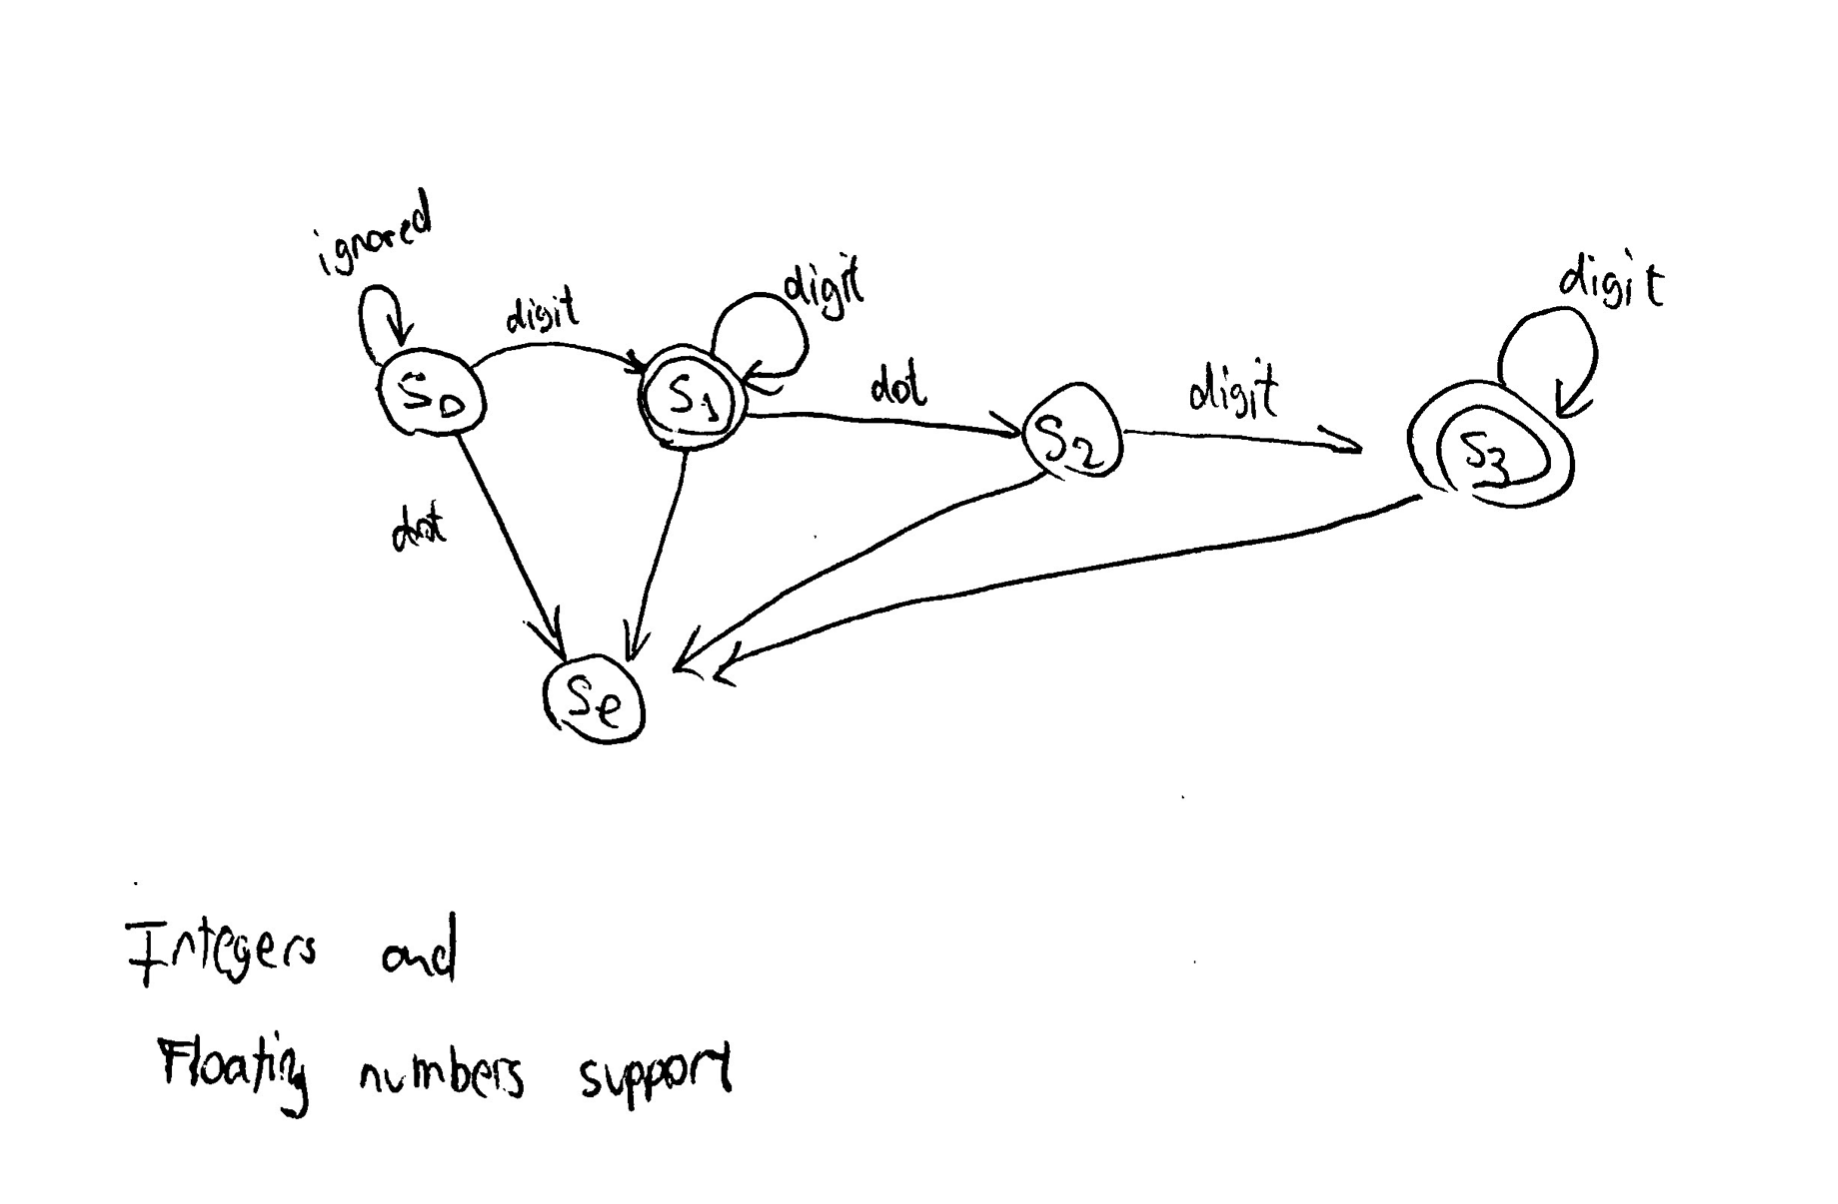
\includegraphics[width=1\textwidth]{images/numbers}}
    \caption{FSA (part concerned with numbers)}
\end{figure}

\begin{figure}[h]
    \centering
    \frame{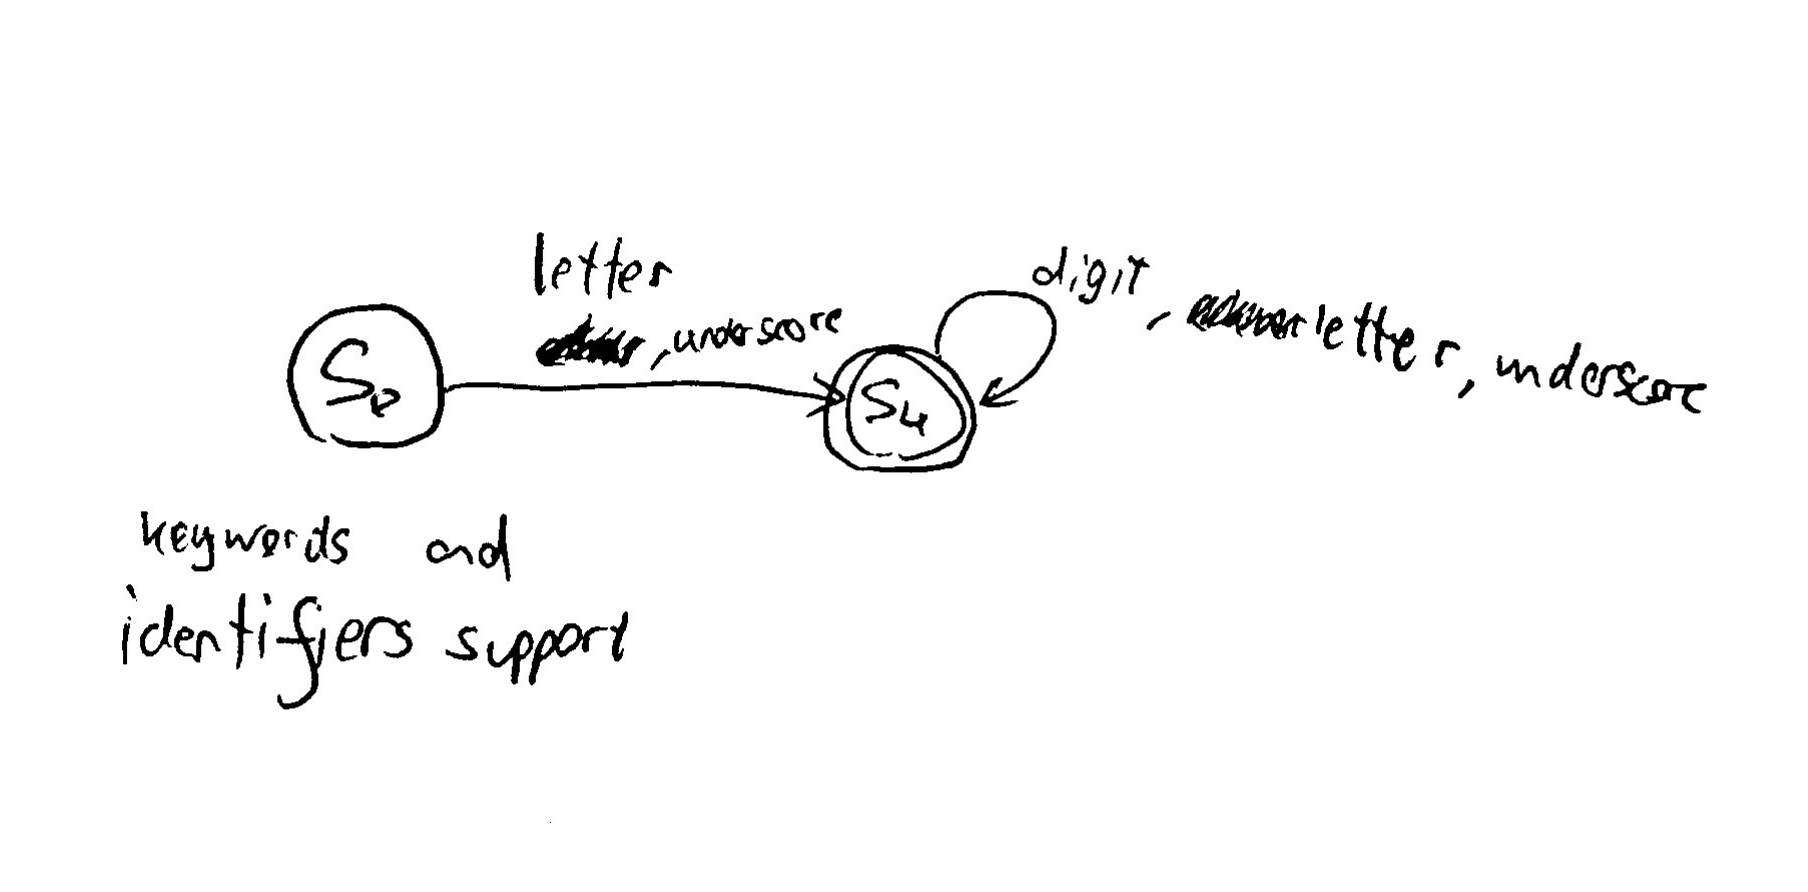
\includegraphics[width=1\textwidth]{images/identifiers}}
    \caption{FSA (part concerned with identifiers and keywords)}
\end{figure}

\begin{figure}[h]
    \centering
    \frame{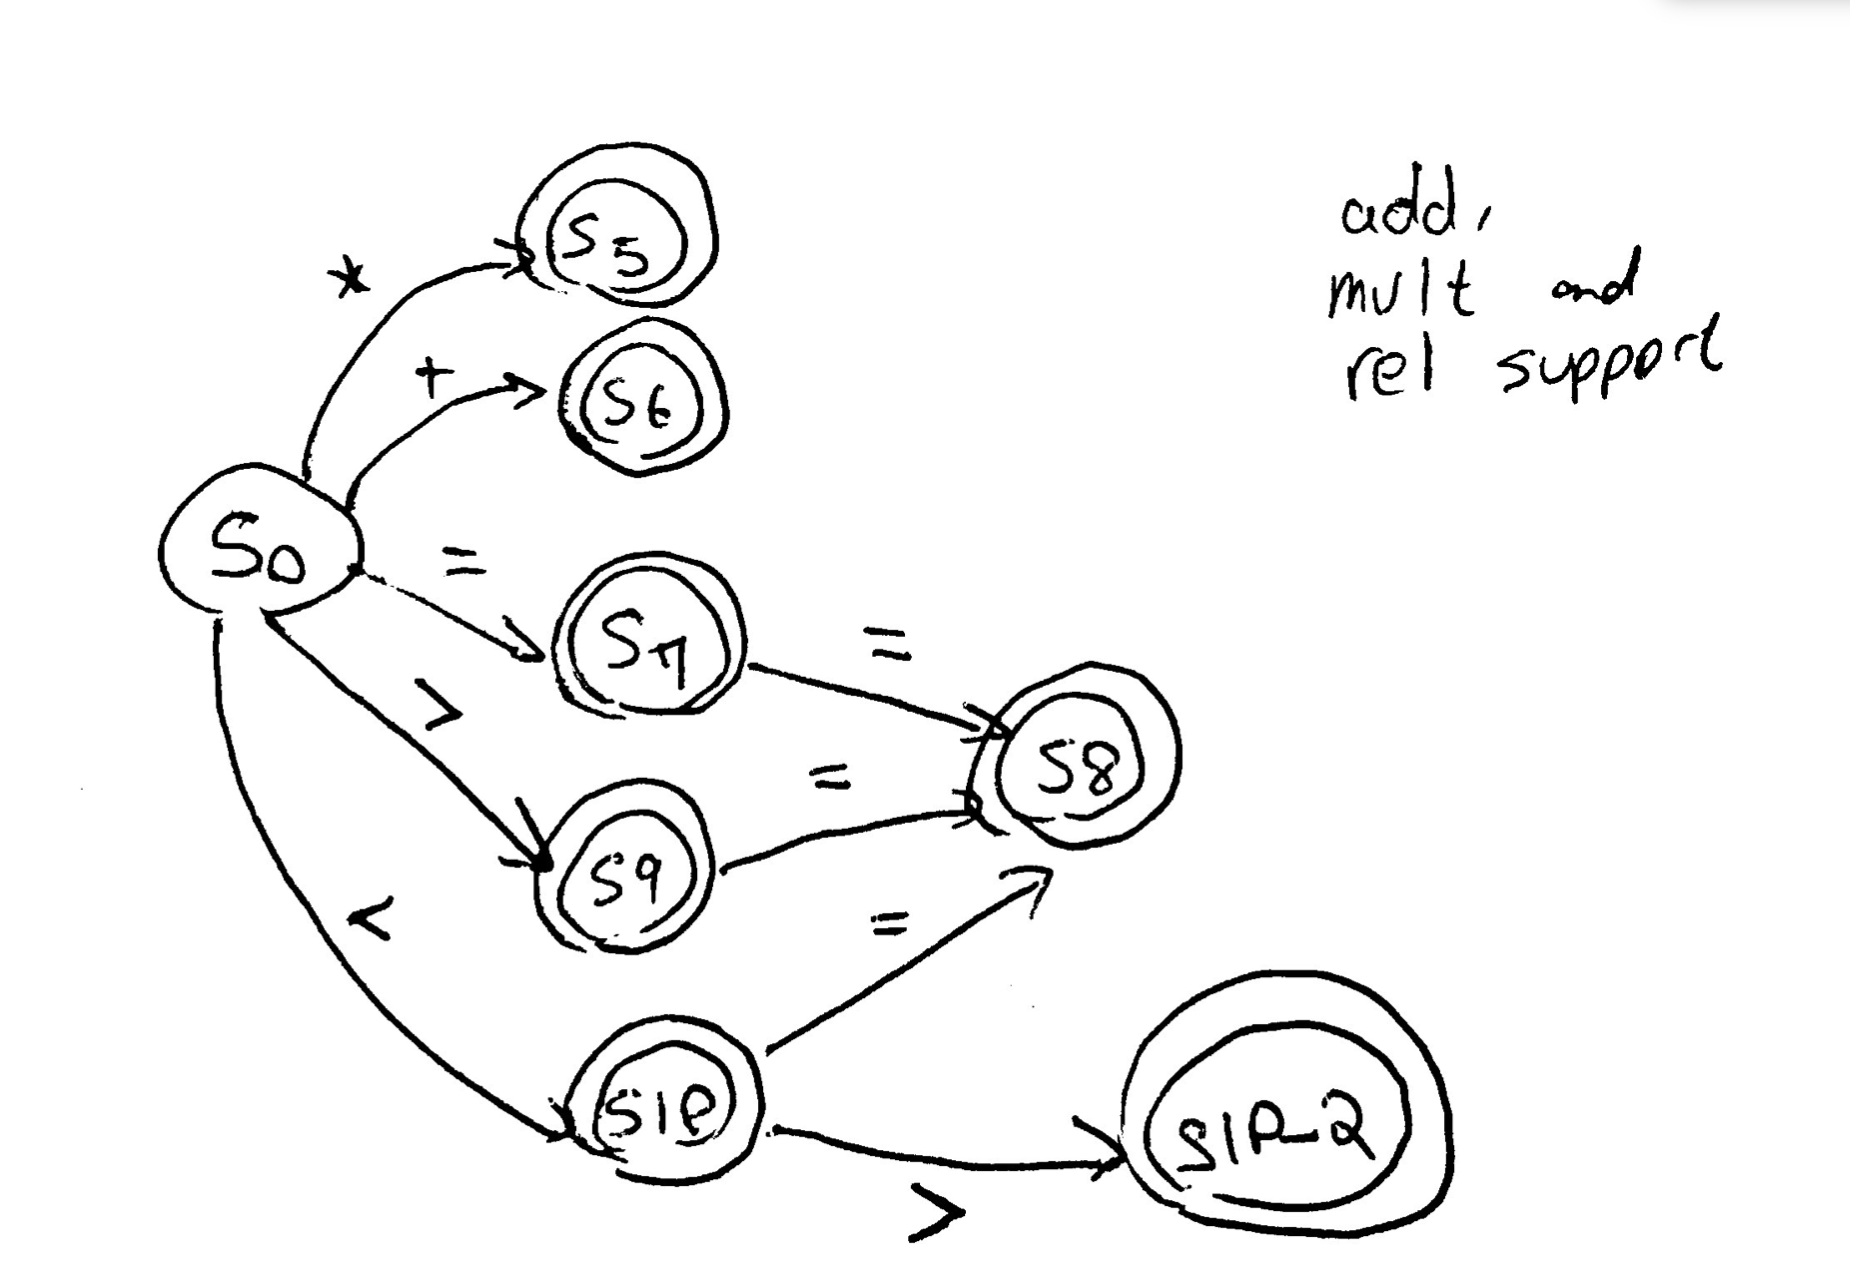
\includegraphics[width=1\textwidth]{images/operators}}
    \caption{FSA (part concerned with operators)}
\end{figure}

\begin{figure}[h]
    \centering
    \frame{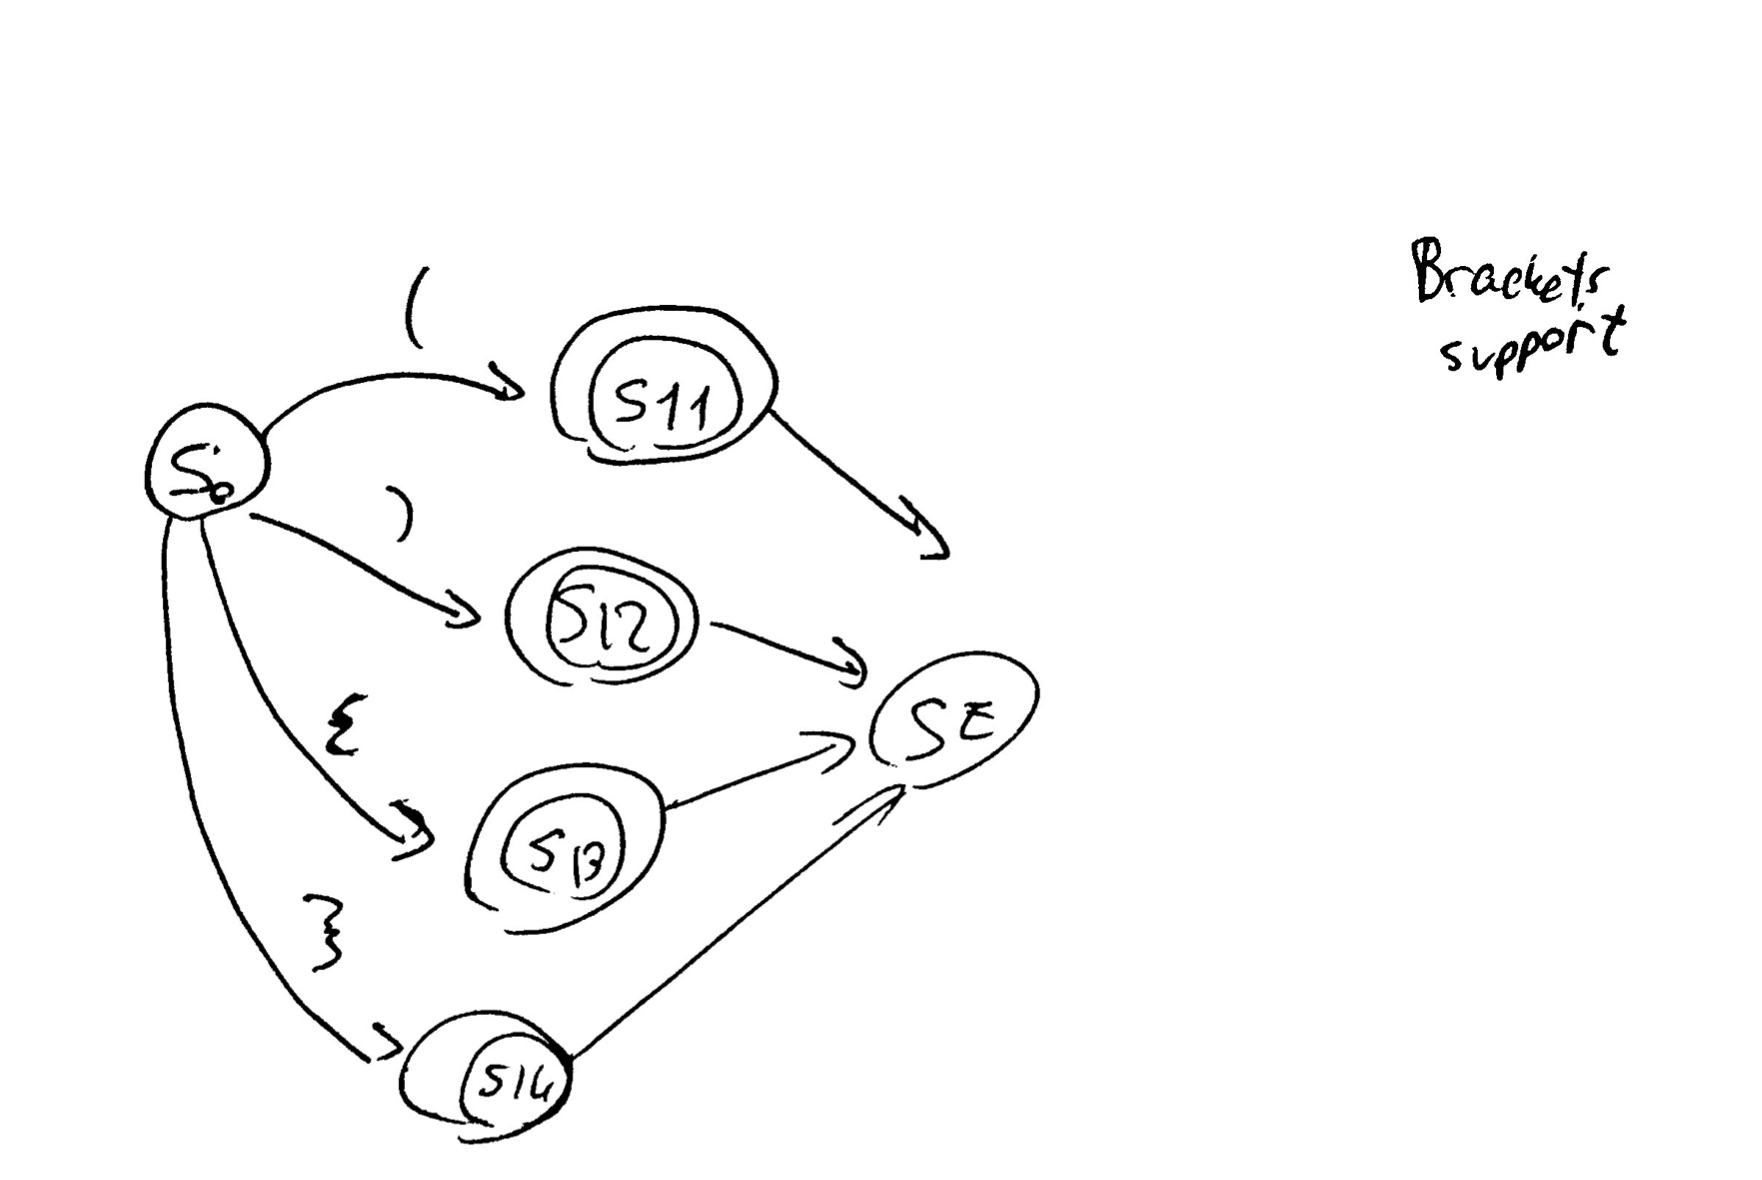
\includegraphics[width=1\textwidth]{images/brackets}}
    \caption{FSA (part concerned with brackets)}
\end{figure}


\begin{figure}[h]
    \centering
    \frame{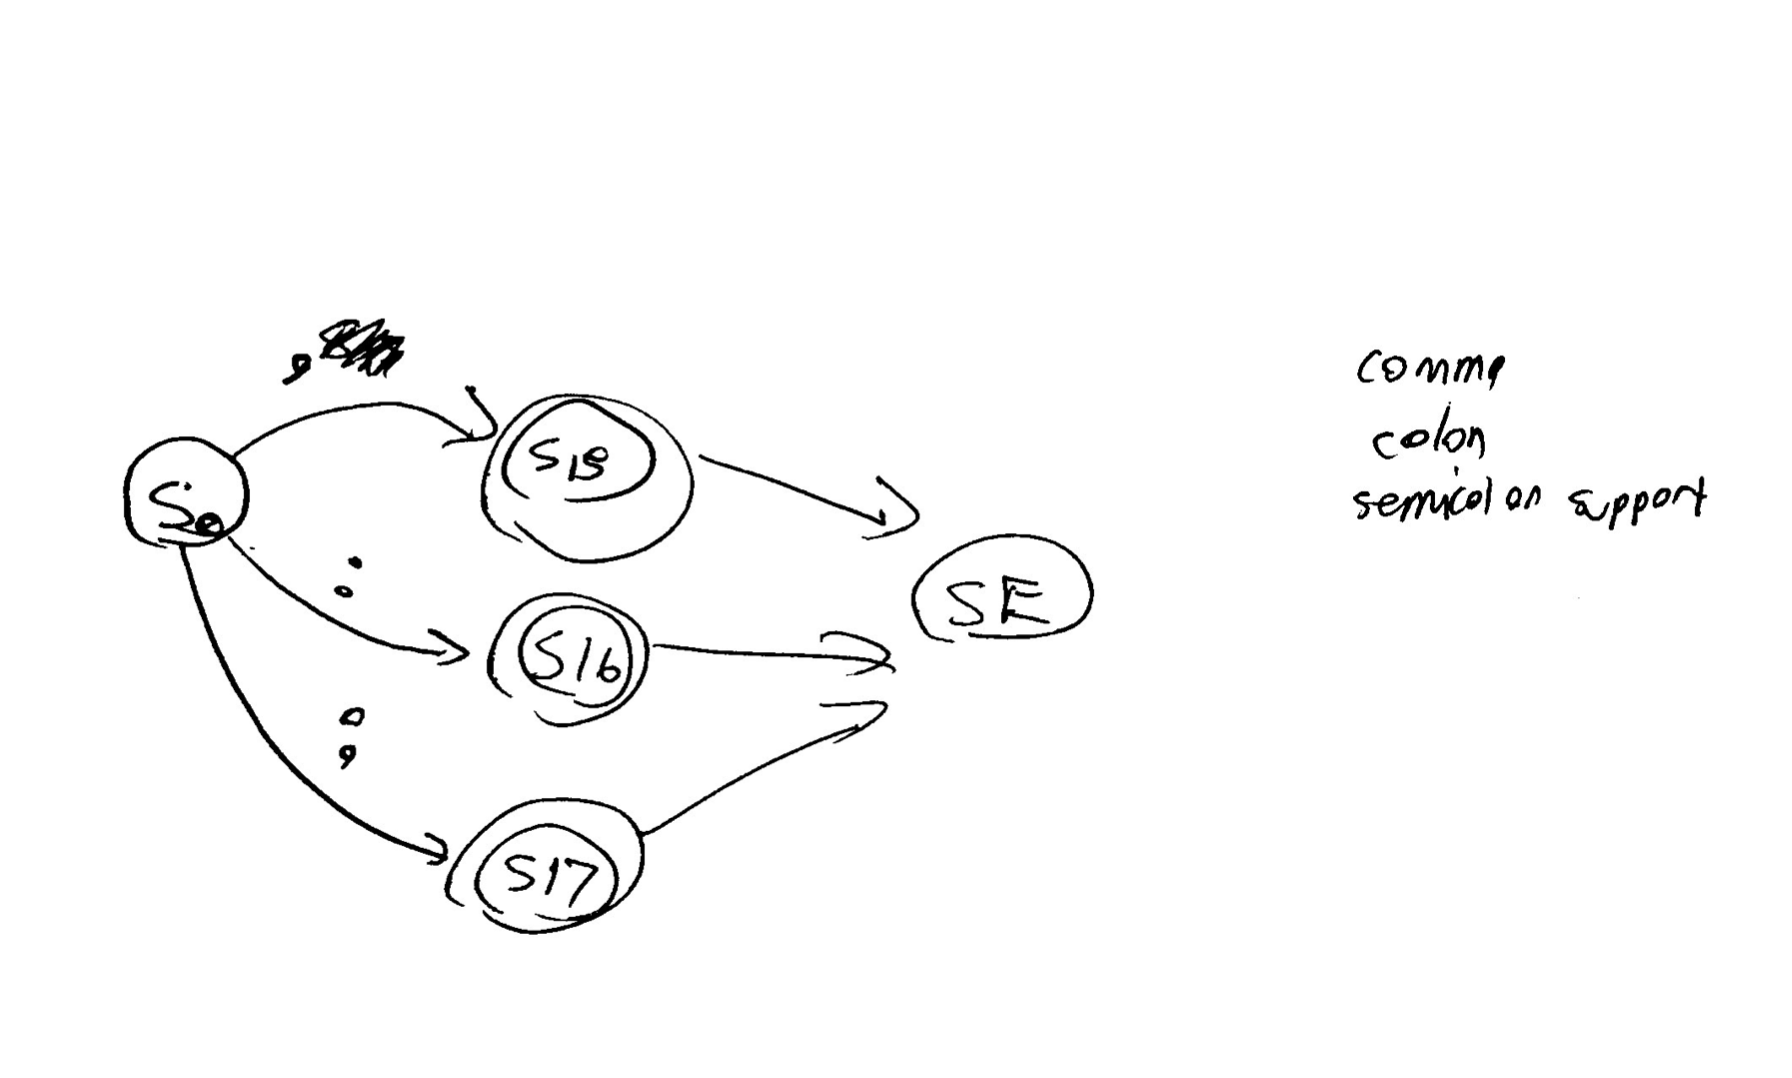
\includegraphics[width=1\textwidth]{images/colons}}
    \caption{FSA (part concerned with colons and comma)}
\end{figure}

\begin{figure}[h]
    \centering
    \frame{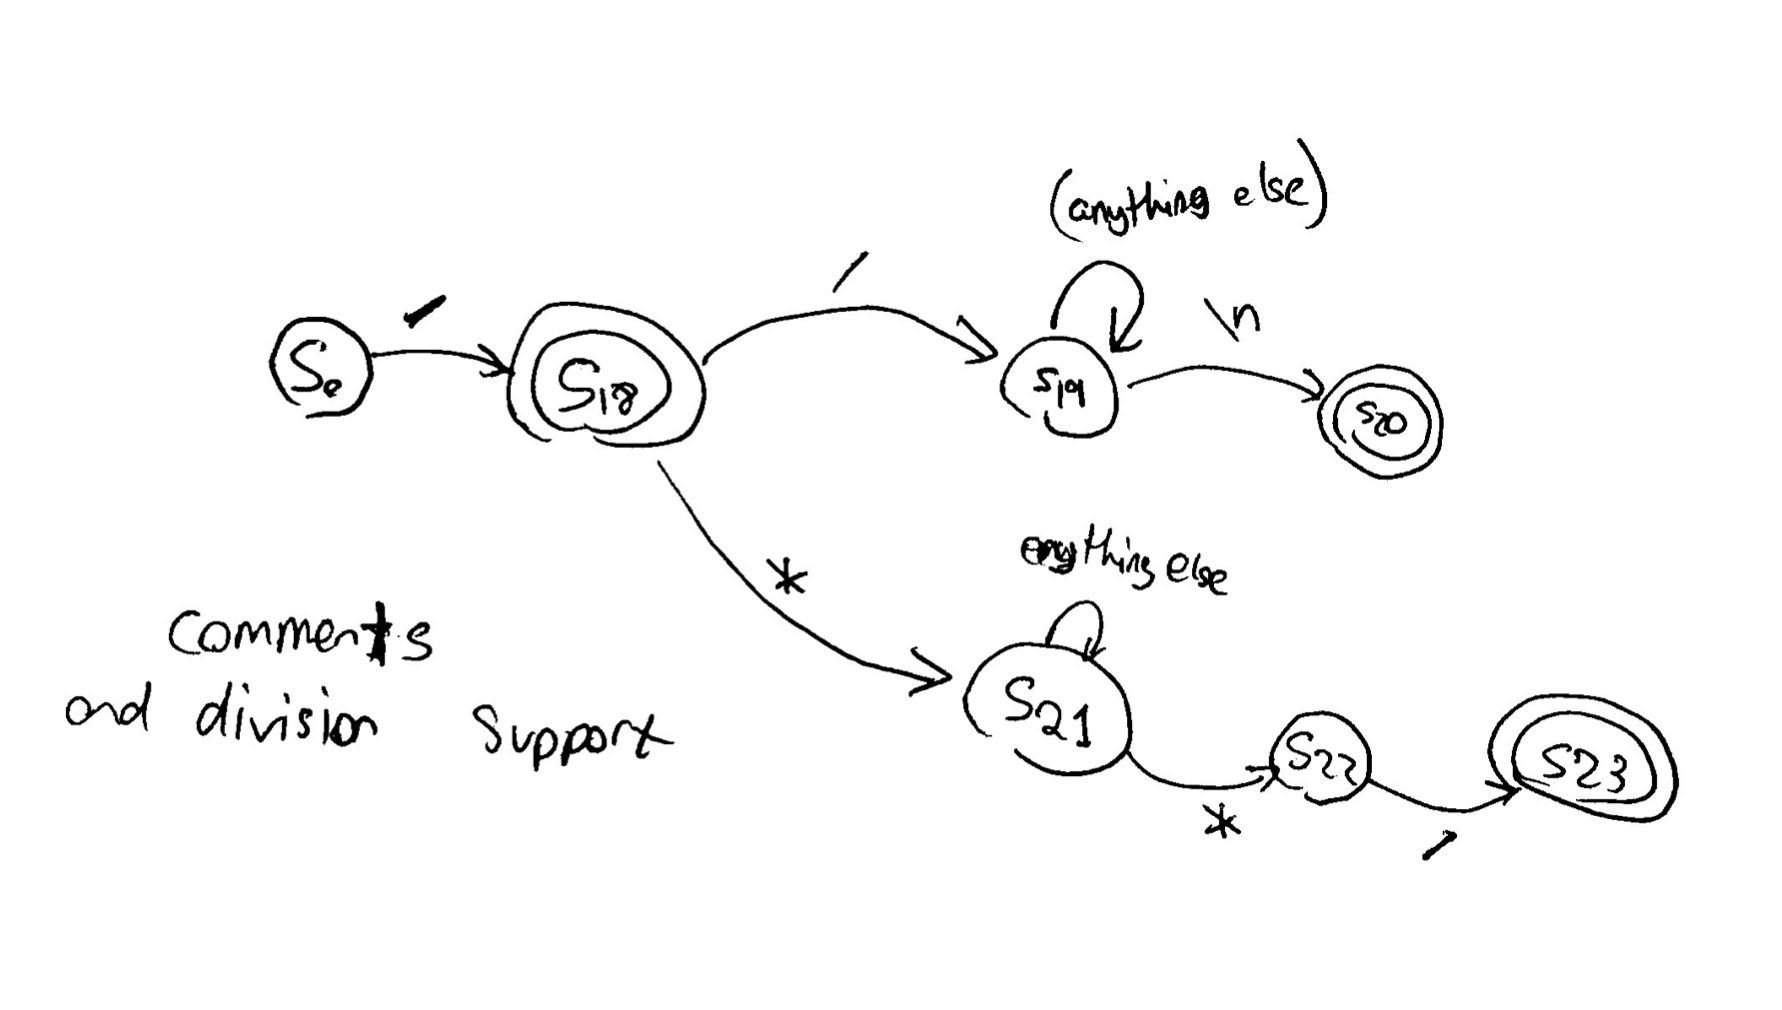
\includegraphics[width=1\textwidth]{images/comments}}
    \caption{FSA (part concerned with comments and division operator}
\end{figure}

\section{Question 2}
\subsection{How the problem was tackled}
For this question, a single path was taken through the EBNF. This path was implemented as boolean functions to test the system.

\begin{lstlisting}[caption="Initial boolean functions"]
bool parse_statement() {
    if ( parse_rtrn_statement() ) {
        if ( parse_semicolon() ) { return true; }
        else { return false; }
    }
    /* TODO: Add other types of statements */

    else { return false; }
}

bool parse_semicolon() {
    if ( tok.type == s_colon ) { tell("semicolon"); advance(); return true; }
    else { return true; }
}

bool parse_rtrn_statement() {
    if ( !parse_return() )     { return false; }
    if ( !parse_expression() ) { return false; }
    return true;
}

bool parse_return() {
    if ( tok.value.compare("return") == 0 ) { tell("return"); advance(); return true; }
    else { return false; }
}
\end{lstlisting}

Later on, a node was declared with binary tree properties. The node holds a token and points to a left node and a right node.
The boolean functions where translated to return a pointer to the node created instead of true and a nullptr instead of false.

\begin{lstlisting}[caption="The change to return node pointer"]
AST* parse_rtrn_statement() {
    tell("rtrn_stmnt");
    AST* rtrn_node = parse_return();
    if ( rtrn_node == nullptr ) {
        return nullptr;
    }

    AST* expression_node = parse_expression();
    if ( expression_node == nullptr ) {
        return nullptr;
    }

    token new_tok;
    new_tok.type = rtrn_statement;
    return make_node(new_tok, rtrn_node, expression_node);
}
\end{lstlisting}

An example of tree building would be the following:
\begin{figure}[h]
    \centering
    \frame{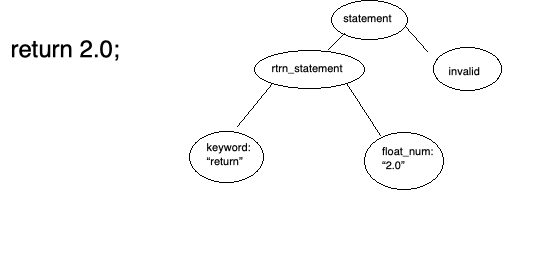
\includegraphics[width=1\textwidth]{images/return_statement_parsing}}
    \caption{Example of AST}
\end{figure}

\subsection{Types of parsing functions}
The section explains how the control forms where implemented within the parsing functions.

\subsubsection{Sequence}
An example from the EBNF that uses sequence is FormalParam. This was implemented by using if statements to and return 
nullptr if the required node is not found.

\begin{lstlisting}[caption="Sequence example"]
AST* parse_rtrn_statement() {
    tell("rtrn_stmnt");
    AST* rtrn_node = parse_return();
    if ( rtrn_node == nullptr ) {
        return nullptr;
    }

    AST* expression_node = parse_expression();
    if ( expression_node == nullptr ) {
        return nullptr;
    }

    token new_tok;
    new_tok.type = rtrn_statement;
    return make_node(new_tok, rtrn_node, expression_node);
}
\end{lstlisting}

\subsubsection{Choice}
Statement is an example that uses choices within the EBNF. These types are implemented by trying to get 
a valid (non nullptr) node. If the function successfully gets a node, it returns the said node in the correct form. If
not (the node was a nullptr) it tries again with the next choice.

\begin{lstlisting}[caption="Choice example"]
AST* parse_statement() {
    tell("statement");
    AST* rtrn_statement_node = parse_rtrn_statement();
    if ( rtrn_statement_node != nullptr ) {
        AST* semicolon_node = parse_semicolon();
        if ( semicolon_node != nullptr ) {
            token new_tok;
            new_tok.type = statement;
            return make_node(new_tok, rtrn_statement_node, semicolon_node);
        }
        else { return nullptr; }
    }

    AST* print_statement_node = parse_print_statement();
    if ( print_statement_node != nullptr ) {
        AST* semicolon_node = parse_semicolon();
        if ( semicolon_node != nullptr ) {
            token new_tok;
            new_tok.type = statement;
            return make_node(new_tok, print_statement_node, semicolon_node);
        }
        else { return nullptr; }
    }

    AST* var_decl_node = parse_var_decl();
    if ( var_decl_node != nullptr ) {
        AST* semicolon_node = parse_semicolon();
        if ( semicolon_node != nullptr ) {
            token new_tok;
            new_tok.type = statement;
            return make_node(new_tok, var_decl_node, semicolon_node);
        }
        else { return nullptr; }
    }

    AST* assignment_node = parse_assignment();
    if ( assignment_node != nullptr ) {
        AST* semicolon_node = parse_semicolon();
        if ( semicolon_node != nullptr ) {
            token new_tok;
            new_tok.type = statement;
            return make_node(new_tok, assignment_node, semicolon_node);
        }
        else { return nullptr; }
    }

    AST* block_node = parse_block();
    if ( block_node != nullptr ) {
        token new_tok;
        new_tok.type = statement;
        return make_node(new_tok, block_node, nullptr);
    }

    AST* while_statement_node = parse_while_statement();
    if ( while_statement_node != nullptr ) {
        token new_tok;
        new_tok.type = statement;
        return make_node(new_tok, while_statement_node, nullptr);
    }

    AST* if_statement_node = parse_if_statement();
    if ( if_statement_node != nullptr ) {
        token new_tok;
        new_tok.type = statement;
        return make_node(new_tok, if_statement_node, nullptr);
    }

    AST* for_statement_node = parse_for_statement();
    if ( for_statement_node != nullptr ) {
        token new_tok;
        new_tok.type = statement;
        return make_node(new_tok, if_statement_node, nullptr);
    }


    AST* func_decl_node = parse_func_decl();
    if ( func_decl_node != nullptr ) {
        AST* semicolon_node = parse_semicolon();
        if ( semicolon_node != nullptr ) {
            token new_tok;
            new_tok.type = statement;
            return make_node(new_tok, func_decl_node, semicolon_node);
        }
        else { return nullptr; }
    }


    else { return nullptr; }
}

\end{lstlisting}
\subsubsection{Options}
Options where implemented by declaring a node but the node doesn't have to be filled. This means the node can be nullptr without
the function quiting.

An example of this is the 'else' part of the if statement.

\begin{lstlisting}[caption="Option example"]
AST* parse_if_statement() { 
    tell("if_statement");  
    AST* if_node = parse_if(); 
    if ( if_node == nullptr)                                            { return nullptr; } 
 
    AST* l_par_node = parse_l_par(); 
    if ( l_par_node == nullptr)                                         { return nullptr; } 
 
    AST* expression_node = parse_expression() ; 
    if ( expression_node == nullptr )                                   { return nullptr; } 
 
    AST* r_par_node = parse_r_par(); 
    if ( r_par_node == nullptr )                                        { return nullptr; } 
 
    AST* block_node = parse_block(); 
    if ( block_node == nullptr )                                        { return nullptr; } 
 
    AST* else_node = parse_else(); 
    AST* else_block_node = parse_block(); 
 
    if ( (else_node == nullptr && else_block_node != nullptr) 
      || (else_node != nullptr && else_block_node == nullptr) )         { return nullptr; } 
 
 
    AST* block = nullptr; 
    token new_tok_0; 
    new_tok_0.type = if_block; 
    block = make_node(new_tok_0, block_node, else_block_node); 
 
    token new_tok_1; 
    new_tok_1.type = if_head; 
    return make_node(new_tok_1, expression_node, block);  
}
\end{lstlisting}

\subsubsection{Repetition}
Repetition is the most complex of the control forms. A recursive function was developed for the tree to add a node to the rightmost.
This enables oarsing functions to add elements to the rightmost node of the tree from an iterative loop.
An example of repetition is the simple expression.

\begin{lstlisting}[caption="Repetition example"]
AST* parse_simp_expression() {
    tell("simp");
    AST* term_node_l = parse_term();
    if ( term_node_l == nullptr )                { return nullptr; }

    AST* add_op_node        = nullptr;
    AST* term_node_r        = nullptr;
    AST* temp_add_op_node   = nullptr;
    AST* temp_term_node_r   = nullptr;

    for(int i=0;; ++i) {
        temp_add_op_node = parse_add_op();
        if ( temp_add_op_node == nullptr )            { break; }

        temp_term_node_r = parse_term();
        if ( temp_term_node_r == nullptr )            { return nullptr; }

        if ( i==0 ) {
            add_op_node = temp_add_op_node;
        }
        add_to_rightmost(term_node_r, temp_add_op_node, temp_term_node_r);
    }

    if ( add_op_node == nullptr ) {
        return term_node_l;
    }

    return make_node(add_op_node->data, term_node_l, term_node_r);
}
\end{lstlisting}

\subsection{Types of nodes}
The way the node was implemented, only a binary tree can be built. Therefore a problem arose for EBNF statements like FuncDecl 
or ForStatements since they contain to much information to be stored in just two child nodes. The workaround used is by creating
a sub tree as a node for the statement. The tree structure of FuncDecl, IfStatement and ForStatement is included with the special nodes
marked with double circles.

\begin{figure}[h]
    \centering
    \frame{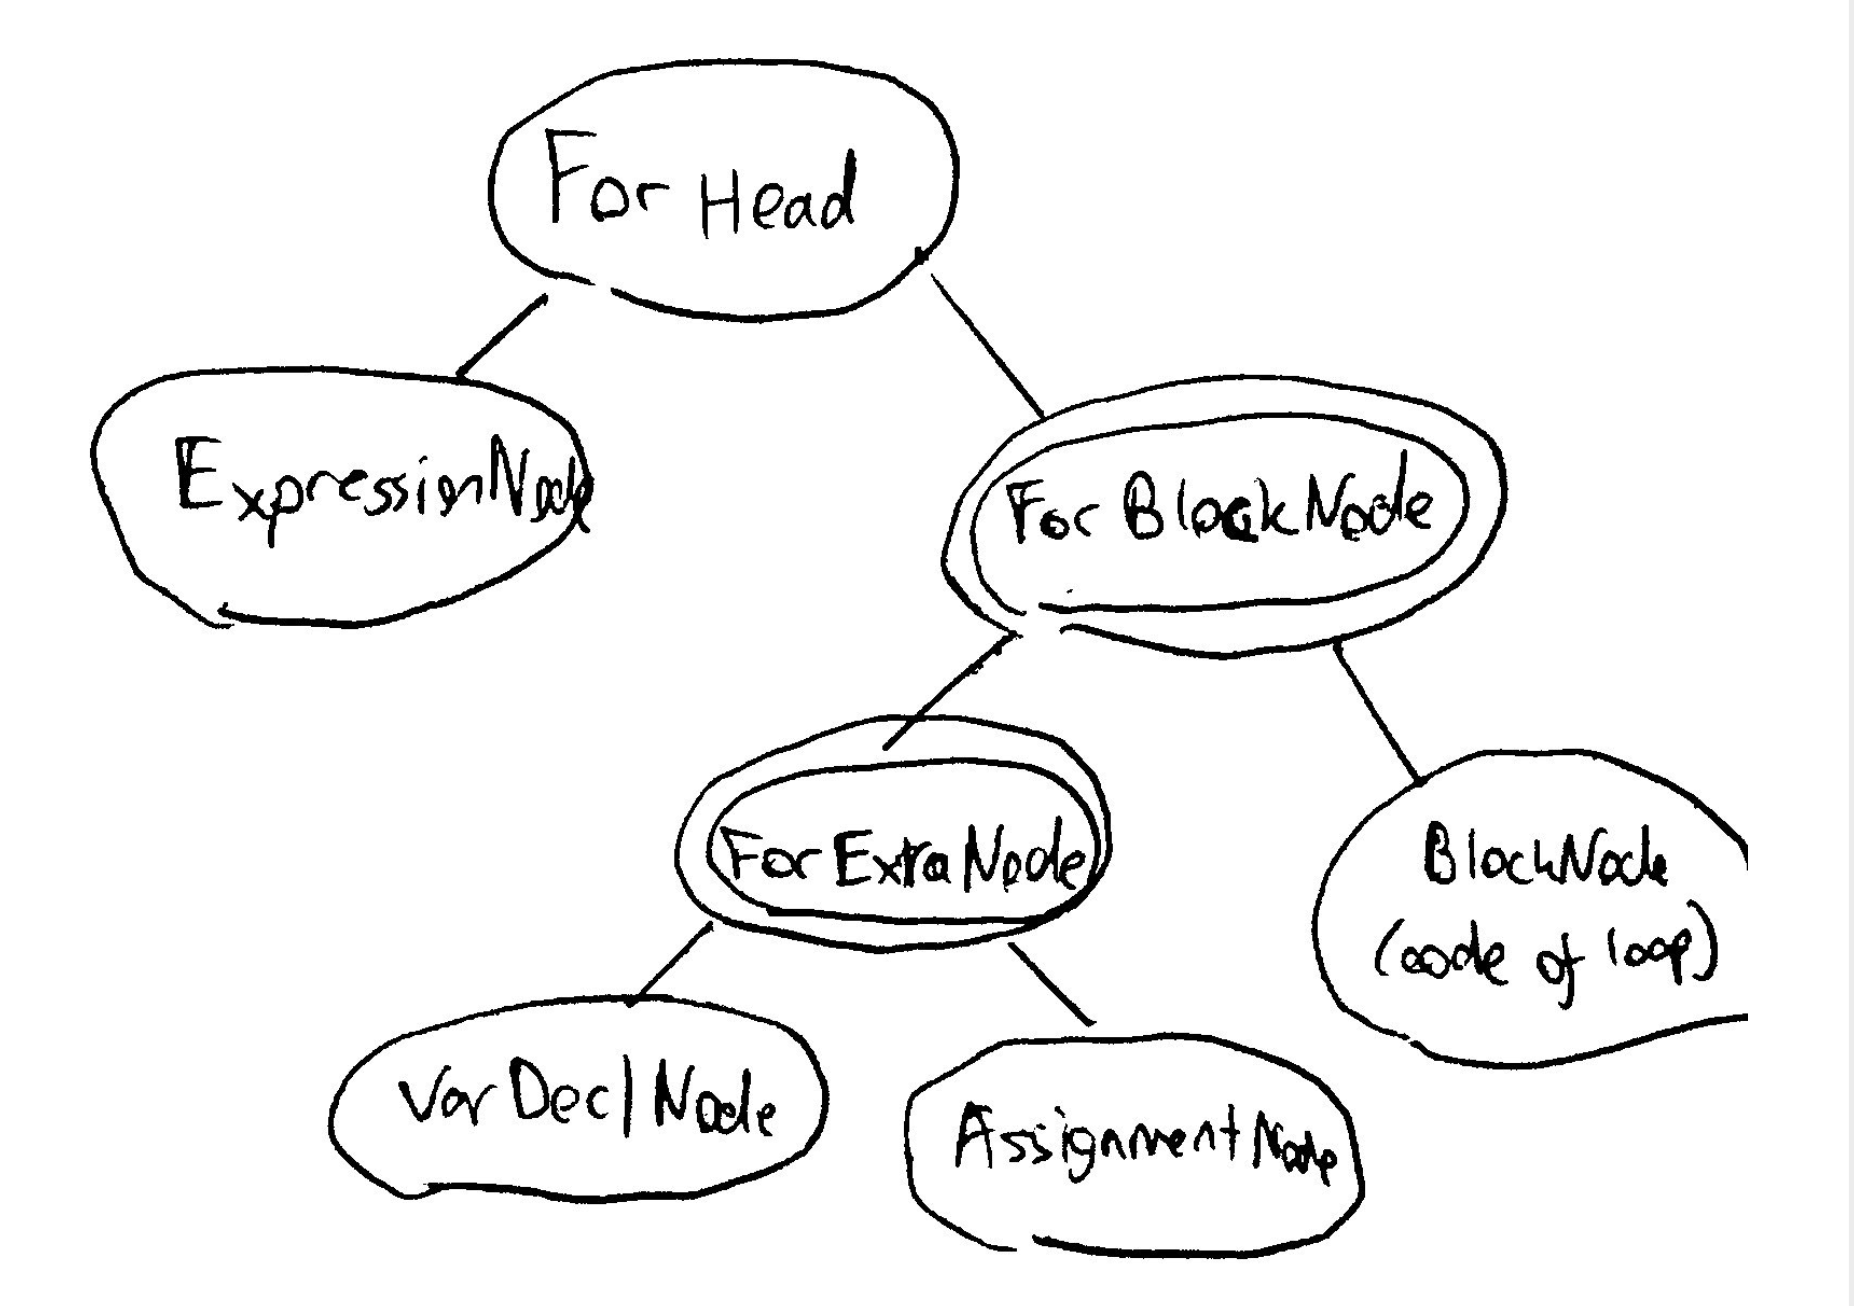
\includegraphics[width=1\textwidth]{images/for_tree}}
    \caption{Tree for ForStatement}
\end{figure}

\begin{figure}[h]
    \centering
    \frame{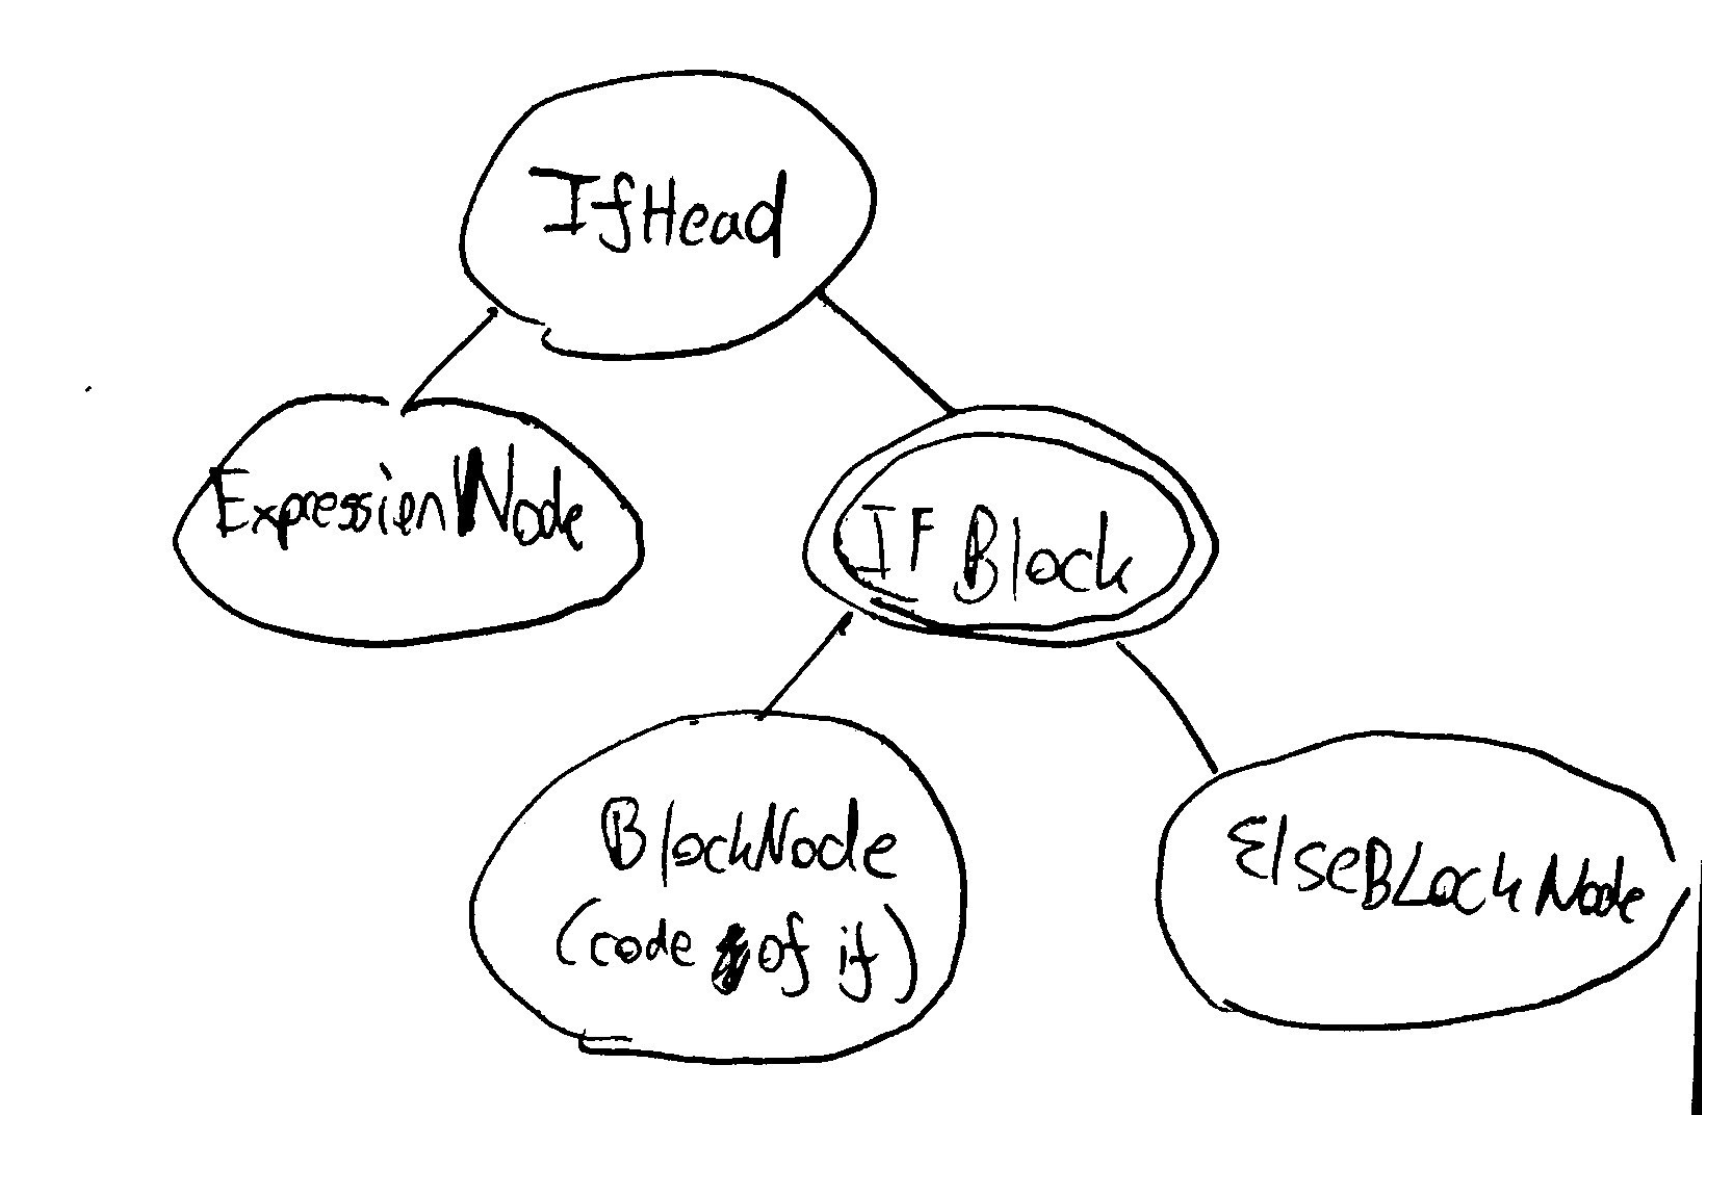
\includegraphics[width=1\textwidth]{images/if_tree}}
    \caption{Tree for IfStatement}
\end{figure}

\begin{figure}[h]
    \centering
    \frame{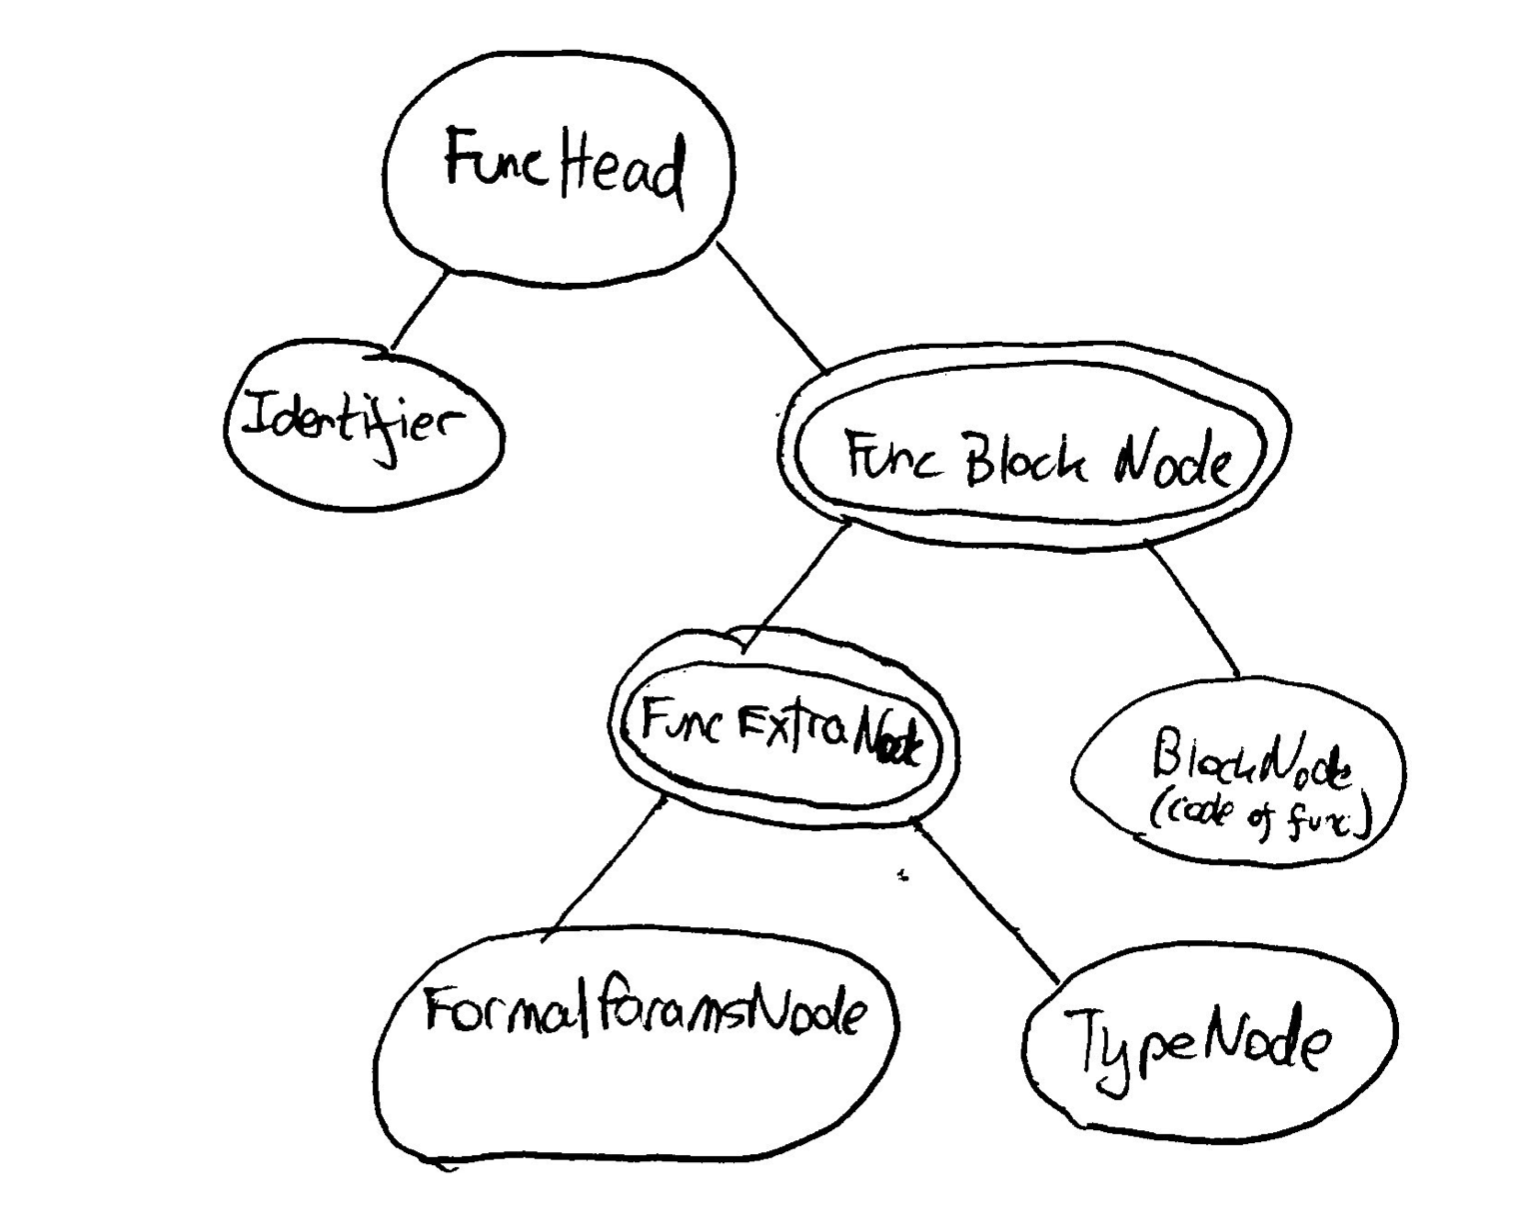
\includegraphics[width=1\textwidth]{images/func_tree}}
    \caption{Tree for FuncDeclStatement}
\end{figure}

\section{Appendix}

\end{document}
